\chapter[ADNEX model systematic review and meta-analysis]{The ADNEX risk prediction model for ovarian cancer diagnosis: A systematic review and meta-analysis of external
validation studies}
% Only include if the thesis is written as a collection of papers
%_________________________
\includegraphics*[width=0.8\linewidth]{logos/BMJ_Medicine.png}
\label{sec:chp_ADNEXSR}

\glsunset{ADNEX}
\glsunset{AUC}
\glsunset{CHARMS}
\glsunset{CI}
\glsunset{CrI}
\glsunset{ESGE}
\glsunset{ESGO}
\glsunset{GRADE}
\glsunset{IOTA}
\glsunset{ISUOG}
\glsunset{JAGS}
\glsunset{NB}
\glsunset{OSF}
\glsunset{PI}
\glsunset{PRISMA}
\glsunset{PROBAST}
\glsunset{QUADAS}
\glsunset{ROC}
\glsunset{RU}
\glsunset{TRIPOD}


published as: 
\begin{quote}
 \textbf{Barreñada L}, Ledger A, Dhiman P et al. ADNEX
risk prediction model for diagnosis of ovarian cancer: systematic review and
meta-analysis of external validation studies. \textit{BMJ Medicine}. 2024;3:e000817. \url{https://doi.org/10.1136/bmjmed-2023-000817}

\end{quote}
\begin{quote}
 \textbf{Supplementary material and code} available in the online version and at \url{https://osf.io/jtsvd/}.
\end{quote}
\vspace{-0.5em}
\noindent\scriptsize\textit{Submitted: 17/11/2023 \quad Published: 17/02/2024 \quad (123 days) \quad APC: 3580 \pounds}
\normalsize\vspace{-0.5 em}
%_________________________
\section*{Summary}
We conducted a systematic review and meta-analysis of 47 studies externally validating the model for ovarian cancer diagnosis in more than 17,000 tumours. 91\% of validations were at high risk of bias, mainly due to the unexplained exclusion of incomplete cases, low sample size, or absent calibration assessment and methodological reporting was poor. The model performed well to distinguish benign from malignant tumours in populations from different countries and settings regardless of whether CA125 was used or not. A key limitation is that calibration was rarely assessed. 

\newpage

\section{Introduction}

The optimal management of patients with an ovarian mass depends on the histology
of the mass. Patients with a benign mass can be managed non-surgically with
clinical and ultrasound follow-up or using conservative surgical techniques 
 \cite{carleyLaparoscopyLaparotomyManagement2002,
froymanRiskComplicationsPatients2019}.
Malignant tumours benefit from management in specialised oncology centres, but
borderline malignancies, stage I primary invasive tumours, and advanced primary
invasive tumours may require different surgical approaches
 \cite{wooCentralisationServicesGynaecological2012,
timmermanESGOISUOGIOTA2021}.
To optimise patient triage without operating on all masses, diagnostic models
can be used to estimate the likelihood of malignancy and so be used to plan
treatment for patients.

Given the potential advantages of accurately predicting risk of malignancy, the
International Ovarian Tumour Analysis (\gls{IOTA}) group developed the Assessment of
Different NEoplasias in the adneXa (\gls{ADNEX}) risk prediction model, using three
clinical and six ultrasound predictor variables
 \cite{vancalsterEvaluatingRiskOvarian2014}. The clinical variables are age,
serum CA-125 level, and type of centre (oncology centre vs other). An oncology
centre is defined as a tertiary referral centre with a specific gynaecology
oncology unit. The ultrasound variables are the maximal diameter of the lesion,
proportion of solid tissue (defined as the largest diameter of the largest solid
component divided by the largest diameter of the lesion), number of papillary
projections, presence of more than 10 cyst locules, presence of acoustic
shadows, and ascites.

\gls{ADNEX} is a multinomial logistic regression model that estimates the risk of five
tumour types: benign, borderline, stage I primary invasive, stage II-IV primary
invasive, and secondary metastatic. The total risk of malignancy calculated by
\gls{ADNEX} is the sum of the risks for each malignant subtype. \gls{ADNEX} has two
versions: one with and one without CA125 as a predictor (the \gls{ADNEX} formulas are
provided in Supplementary material S1)
 \cite{vancalsterEvaluatingRiskOvarian2014}. When we refer to ‘the \gls{ADNEX} model’
or “\gls{ADNEX}”, we refer to both versions of the model. The model was developed on
data from 5909 patients with an adnexal mass that subsequently underwent surgery
and that were recruited at 24 centres across 10 countries (Belgium, Italy, Czech
Republic, Poland, Sweden, China, France, Spain, UK and Canada). Although
developed on data from patients that underwent surgery, the performance of \gls{ADNEX}
has been evaluated also on cohorts that included non-surgically managed patients
 \cite{vancalsterValidationModelsDiagnose2020,
hackExternalValidationORADS2022,
jeongValidationIOTAADNEXModel2020,
quarantaSurgeryBenignOvarian2020}.

\gls{ADNEX} is included in national guidelines, e.g. in Belgium, The Netherlands and
Sweden
 \cite{RegionalaCancercentrumSamverkan2023,
ignaceEierstokkankerDiagnoseBehandeling2016,geominipZonMwProjACCEPTAccuracy2021}.
It is recommended by scientific societies, such as International Society of
Ultrasound in Obstetrics and Gynecology (\gls{ISUOG}), European Society of
Gynaecological Oncology (\gls{ESGO}), European Society for Gynaecological Endoscopy
(\gls{ESGE}), and the American College of Radiology
 \cite{timmermanESGOISUOGIOTA2021,
andreottiORADSUSRisk2020}. In addition,
manufacturers of ultrasound machines have begun to incorporate \gls{ADNEX} directly
into their machines.

Several external validation studies of \gls{ADNEX} have been carried out. To date,
five published systematic reviews and meta-analyses of \gls{ADNEX} have summarised
between 3 and 22 external validation studies
 \cite{cuiDiagnosticAccuraciesUltrasound2022,
davenportMenopausalStatusUltrasound2022,
huangDiagnosticAccuracyADNEX2021,
westwoodRiskScoresGuide2018,
yueValueAssessmentDifferent2022}.
All systematic reviews evaluated \gls{ADNEX} solely as a diagnostic test, reporting a
summary sensitivity and specificity at a threshold for the estimated risk of
malignancy of 10\% or 15\%
 \cite{cuiDiagnosticAccuraciesUltrasound2022,
davenportMenopausalStatusUltrasound2022,
huangDiagnosticAccuracyADNEX2021,
westwoodRiskScoresGuide2018,
yueValueAssessmentDifferent2022}.
However, the \gls{ADNEX} model is not only a test to classify masses as benign or
malignant. It is a risk prediction model to provide probability estimates of
five different tumour types at the individual patient level. Only focusing on
classification performance leads to a loss of useful information
 \cite{onbehalfofthetopicgroupevaluatingdiagnostictestsandpredictionmodelsofthestratosinitiativeThreeMythsRisk2019}.
When validating \gls{ADNEX} as a diagnostic test at a 10\% threshold, the performance
metrics (i.e. sensitivity/specificity) do not take into account the individual
risks predicted but the same weight is given to a misclassified patient with
11\% risk as with 99\% risk. This means that these meta-analyses have not fully
validated the diagnostic performance of \gls{ADNEX}. For example, pooling
discrimination performance (area under the receiver operating characteristic
curve, \gls{AUC}) allows us to determine the ability of the model to differentiate
between patients with and without the outcome across different thresholds.

There are now guidelines on how to evaluate the quality and risk of bias of
external validation studies of risk prediction models
 \cite{debrayGuideSystematicReview2017,
wolffPROBASTToolAssess2019,
snellTransparentReportingMultivariable2023}.
These should be used in meta-analyses of validation studies. The objective of
this study is to conduct a systematic review of studies that externally validate
\gls{ADNEX}, to describe reporting completeness and risk of bias of the validation
studies, and to conduct meta-analyses of model performance measures.

\section{Methods}

\subsection{Protocol registration}
We report this study according to the \gls{PRISMA} (Preferred Reporting Items for
Systematic reviews and Meta-Analysis) and \gls{TRIPOD}-SRMA (Transparent Reporting of
multivariable prediction models for Individual Prognosis Or Diagnosis: checklist
for Systematic Reviews and Meta-Analyses) checklists
 \cite{snellTransparentReportingMultivariable2023,
pagePRISMA2020Statement2021}.
The study protocol was prospectively registered in the International prospective
register of systematic reviews (PROSPERO; ID CRD42022373182).

\subsection{Eligibility criteria}
Any study that carried out an external validation to evaluate the performance of
the \gls{ADNEX} model using any study design and any study population was eligible for
inclusion in the systematic review. The exclusion criteria were (1) studies that
did not evaluate the model performance of \gls{ADNEX} in any way; (2) studies that
evaluated the predictive performance only of updated versions of \gls{ADNEX}; (3)
studies for which only an abstract is available, or the full text cannot be
obtained; (4) case studies presenting \gls{ADNEX} performance for individual patients
(this criterion was not pre-specified in the protocol but was added post hoc
upon review of the search results). Updating can refer to recalibration,
refitting, or extension with additional predictors
 \cite{steyerbergClinicalPredictionModels2009}. Studies that conduct comparisons
of \gls{ADNEX} with other models reporting performance metrics are similarly eligible
for inclusion.

\subsection{Information sources and search strategy}
We created a search string and overall search strategy with the help of
biomedical reference librarians of the KU Leuven Libraries. We searched the
electronic databases Medline (via PubMed), EMBASE, Web of Science, and Scopus
for published articles, and EuropePMC for preprints. The search dates were from
the publication of the first \gls{ADNEX} paper (15/10/2014) until 15/05/2023 (date the
final search was run). We also screened all articles citing the original \gls{ADNEX}
paper \cite{vancalsterEvaluatingRiskOvarian2014}. The reference lists of
relevant review and opinion articles retrieved by the search strings were
checked for other potentially eligible articles. Forward and backward
snowballing (forward/back cross-reference checking) of the included articles was
performed to identify additional publications
 \cite{wohlinGuidelinesSnowballingSystematic2014}. There was no language
restriction, but for papers in languages other than English, Spanish, Dutch,
French or Swedish an automatic translation tool (deepl.com) was used to decide
whether to include or exclude a paper and to extract information. The full
search strategy is provided in Supplementary Material S2.

\subsection{Study selection}
The studies we identified in our search were imported into Zotero reference
manager, where they were automatically de-duplicated. The de-duplicated records
were then imported into Rayyan web application for manual de-duplication (LB)
and subsequent screening of title and abstract by two independent authors with
any conflicts being resolved by discussions between them (LB, AL)
 \cite{ouzzaniRayyanWebMobile2016}.

As three authors (BVC, LV, DT) are members of the \gls{IOTA} group that developed
\gls{ADNEX}, we separated the studies as linked or not linked to \gls{IOTA}. A study was
\gls{IOTA}-linked if it was co-authored by a member of the \gls{IOTA} steering committee
(Supplementary Material S3). \gls{IOTA}-linked papers, as well as a few others with a
potential conflict of interest (i.e., including authors that are or were \gls{IOTA}
collaborators), were independently assessed by authors PD and GSC, two medical
statisticians with expertise in prediction modelling and unrelated to \gls{IOTA}. All
other studies were independently assessed by authors LB and AL. Conflicts were
resolved through discussion between reviewers and for the non-\gls{IOTA} papers also
through discussion with authors BVC, LV and JYV.

\subsection{Data extraction and data items}
Data was extracted and entered into a standardised data extraction form in
Microsoft Excel. The data extraction focused on general and design
characteristics of studies, target population, reference standard, sample size,
performance results, reporting quality, methodological quality, and risk of bias
(Table S1). The extraction form was based on and adapted from the \gls{CHARMS}
(CHecklist for critical Appraisal and data extraction for systematic Reviews of
prediction Modelling Studies), \gls{TRIPOD} (Transparent Reporting of a multivariable
prediction model for Individual Prognosis Or Diagnosis), and \gls{PROBAST} (Prediction
model Risk Of Bias ASsessment Tool) tools
 \cite{wolffPROBASTToolAssess2019,
moonsCriticalAppraisalData2014,
collinsTransparentReportingMultivariable2015}.

To describe model performance, we extracted information on any reported measure
related to discrimination, calibration, diagnostic accuracy, or clinical
utility. The reference standard could be binary (e.g., benign vs malignant) or
multinomial (e.g., the five tumour types predicted by \gls{ADNEX}). Performance data
was extracted for all reported validations (i.e., for both \gls{ADNEX} with and
without CA125), subgroup analyses, sensitivity analyses, and centre-specific
results in multicentre studies.

For each study we assessed the reporting of all \gls{TRIPOD} items that are applicable
to external validation studies (Table S2). We also checked \gls{PROBAST}’s ‘signalling
questions’ and evaluated risk of bias for each subdomain (participants,
predictors, outcome, and analysis) and overall. We included rationale for the
risk of bias classification. We contacted study authors to obtain further
information or results in the following situations: (1) when centre-specific
results were not reported in multicentre studies, (2) the type of centre was not
explicitly reported (in case of nonresponse, the clinical co-authors, JYV, DT,
and LV, classified the centre), (3) overall performance was reported but not
performance by menopausal status, or (4) performance was not reported for
operated patients separately in studies including both surgically and
non-surgically managed patients. Details on all extracted items are available in
Supplementary Material (Table S1) and Open Science Framework repository
(Extraction sheet) \cite{barrenadaADNEXRiskModel2025}.

\subsection{Statistical analysis and quantitative data synthesis}
Data were summarised with descriptive statistics and data visualisations.
Meta-analysis of performance, using centre-specific results for multicentre
studies where possible, was performed using random effects meta-analysis
methods. Meta-analysis was done separately for \gls{ADNEX} with and without CA125. In
addition to 95\% confidence intervals (\gls{CI}) for the summary performance, we
assessed heterogeneity using tau squared and 95\% prediction intervals (\gls{PI}).
Supplementary Material S4-S6 provides details on the statistical methodology,
including meta-analysis methods, explanations of Net Benefit and Relative
Utility, and publication bias assessment.

Meta-analysis of the \gls{AUC} for benign versus malignant tumours was done on the
logit scale. Meta-analysis for sensitivity and specificity was also performed on
the logit scale using random effects meta-analysis
 \cite{rileyBivariateRandomeffectsMetaanalysis2007}. As the meta-analysis was
only conducted for the 10\% threshold for the risk of malignancy we did not need
the 95\% confidence ellipse in \gls{ROC} space, so we did not use the bivariate random
effects model as specified in the protocol. The 10\% threshold was most commonly
used in the articles included in our systematic review, and is a commonly
recommended threshold \cite{timmermanESGOISUOGIOTA2021}. Meta-analysis of Net
Benefit (\gls{NB}) \cite{vickersDecisionCurveAnalysis2006} and Relative Utility (\gls{RU})
 \cite{bakerPuttingRiskPrediction2009} at the 10\% risk of malignancy threshold
was performed using Bayesian trivariate random effects meta-analysis of
sensitivity, specificity and prevalence of malignancy
 \cite{wynantsRandomeffectsMetaanalysisClinical2018}. For Bayesian methods, 95\%
credible intervals (\gls{CrI}) are reported instead of 95\% \glspl{CI}. The Bayesian approach
allowed to estimate the probability that the model is useful in a new center,
i.e. the probability that \gls{RU} is >0.

To address multinomial discrimination performance, meta-analysis of \glspl{AUC} between
pairs of tumour outcomes (‘pairwise \glspl{AUC}’) was conducted on logit scale. We only
included studies that used the “conditional risk method” to calculate pairwise
\glspl{AUC} \cite{vancalsterAssessingDiscriminativeAbility2012}. Subgroups are defined
based on geographical location, type of centre, and menopausal status.
Sensitivity analyses are based on the risk of bias judgment and on whether the
study was \gls{IOTA} linked or not. As pre-specified in the protocol, we only
meta-analysed performance if at least three estimates in a specific analysis
could be retrieved from the included studies. To assess the association of
prevalence of malignancy with the \gls{AUC} and sensitivity and specificity at the
10\% risk of malignancy threshold, we used meta-regression
 \cite{thompsonHowShouldMetaregression2002}.

Reporting bias and small study effects were visually explored using funnel plots
adapted for the \gls{AUC}. The body of evidence was assessed using an adapted version
of \gls{GRADE} \cite{guyattGRADEEmergingConsensus2008}. All analyses were performed in
R version 4.2.2 using package “metamisc” for the \gls{AUC}, “meta” and “mada” for
sensitivity and specificity, and rjags for \gls{NB} and \gls{RU}
 \cite{debrayFrameworkMetaanalysisPrediction2019,
schwarzerMetaAnalysis2015,
doeblerMetaanalysisDiagnosticAccuracy2025,
plummerRjagsBayesianGraphical2023}.
Bayesian methods were computed using \gls{JAGS} version 4.3.1
 \cite{plummerRjagsBayesianGraphical2023}.

 \begin{table}[h!]
\small
\centering
\caption{Characteristics of the 47 included studies.}
\label{tab:1}
\begin{tabularx}{\linewidth}{l c >{\raggedright\arraybackslash}X}
\toprule
\textbf{Study characteristic} & \textbf{N (\%)} & \textbf{Comments} \\ 
\midrule
\textbf{Unit of analysis} & & \\
\quad Patient & 42 (89) & 1 tumour per patient \\
\quad Tumour & 5 (11) & >1 tumour per patient possible \\
\addlinespace
\textbf{Region} & & \\
\quad Asia & 24 (51) & Common countries: China (12), South Korea (3) \\
\quad Europe & 18 (38) & Common countries: Poland (7), Italy (4), Spain (4), UK (3), Sweden (3) \\
\quad South America & 3 (6) & \\
\quad North America & 2 (4) & \\
\addlinespace
\textbf{Number of centres} & & \\
\quad 1 & 37 (79) & \\
\quad 2-5 & 7 (15) & \\
\quad >5 & 3 (6) & Range: 8-17 \\
\addlinespace
\textbf{Type of centre} & & \\
\quad Oncology centre(s) & 35 (74) & \\
\quad Non-oncology centre(s) & 2 (4) & \\
\quad Both types of centres & 4 (9) & \\
\quad Unclear & 6 (13) & \\
\addlinespace
\textbf{ADNEX version} & & \\
\quad \gls{ADNEX} with CA125 & 37 (79) & 21 only used \gls{ADNEX} with CA125, 16 used both \\
\quad \gls{ADNEX} without CA125 & 19 (40) & 3 only used \gls{ADNEX} without CA125, 16 used both \\
\quad Mixed & 3 (6) & \gls{ADNEX} with CA125 used if CA125 was available \\
\quad  Unclear & 4 (9) & \\
\addlinespace
\textbf{Selection based on histology} & & \\
\quad No & 39 (83) & \\
\quad Yes & 8 (17) & e.g., borderlines excluded, only invasive tumours \\
\addlinespace
\textbf{Focus only on clinical subgroup} & & \\
\quad No & 42 (89) & \\
\quad Yes & 5 (11) & e.g., only pregnant patients \\
\addlinespace
\textbf{Target population} & & \\
\quad Surgically managed patients & 43 (91) & \\
\quad Surgically and non-surgically managed patients & 4 (9) & \\
\bottomrule
\end{tabularx}
\end{table}


\section{Results}

\begin{figure}
\centering
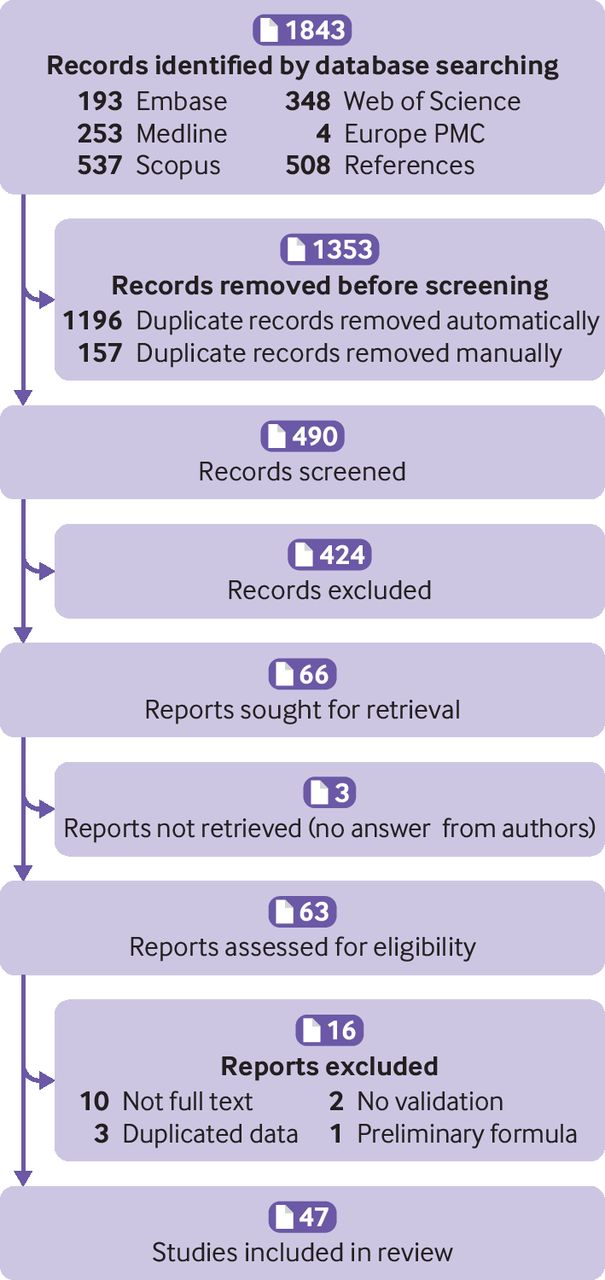
\includegraphics[scale=1]{figures/ADNEXSR/F1.jpg}
\caption[PRISMA flowchart]{PRISMA (Preferred Reporting Items for Systematic Reviews and Meta-Analyses) flowchart of study inclusions and exclusions.}
\label{fig:1:1}
\end{figure}



We identified 1843 records and screened 490 after de-duplication. Forty-seven
studies met our inclusion criteria and were included in this systematic review
(Figure \ref{fig:1:1}, Table S3)
 \cite{vancalsterValidationModelsDiagnose2020,
hackExternalValidationORADS2022,
jeongValidationIOTAADNEXModel2020,
quarantaSurgeryBenignOvarian2020,
araujoPerformanceIOTAADNEX2017,
behnamfarComparisonUltrasoundTumor2022,
budianaSkorAssessmentDifferent2022,
butureanuOvarianMassesapplicableIota2021,
chenComparisonORADSADNEX2022,
chenPerformanceIOTAADNEX2019,
czekierdowskiSonographicAssessmentComplex2021,
czekierdowskiPerformanceIOTASimple2023,
diazOvarianTumorsRisk2017a,
epsteinSubjectiveUltrasoundAssessment2016,
esquivelvillabonaTwoStepStrategyOptimizing2022,
gaurilcikasPerformanceIOTAADNEX2020,
heEstimatingRiskMalignancy2021,
hiettPerformanceIOTASimple2022,
huComparisonUltrasoundbasedADNEX2023,
jiangOvarianSexCord2021,
jianhongComparisonPerformanceORADS2022,
joyeuxSurgeryPredictabilityMalignant2016,
laiComparisonORADSGIRADS2022,
lamhuongOptimalCutOffPoint2022,
leeUltrasonographicEvaluationOvarian2021,
liuADNEXModelbasedDiagnosis2021,
meysEstimatingRiskMalignancy2017,
namAssessmentDifferentNEoplasias2021,
nohuzReliabilityIOTAScore2019,
pelayoComparisonUltrasoundScores2023,
pengEvaluationDiagnosticValue2021,
poonyakanokPreoperativeEvaluationADNEX2021,
qianComparisonDiagnosticPerformances2021,
rashmiDiagnosticPerformanceUltrasoundBased2023,
sandalComparisionRiskMalignancy2018a,
sayasnehEvaluatingRiskOvarian2016,
stukanDevelopmentValidationModel2019,
stukanUltrasoundClinicalPreoperative2019,
szubertExternalValidationIOTA2016,
szubertPerformanceSelectedModels2020,
tavoraiteUltrasoundAssessmentAdnexal2021,
tugPreoperativeDiscriminatingPerformance2020,
velayoDiagnosticPerformancesUltrasoundBased2023,
vioraADNEXModelTriage2020,
wangEvaluatingRiskMalignancy2023,
yangPerformanceIOTAADNEX2022,
zhangExternalValidationAssessment2022}.
Three studies were excluded because they used the same data as in another
included study, and one study was excluded because a preliminary formula of
\gls{ADNEX} was used
 \cite{landolfoBenignDescriptorsADNEX2023,
poonyakanokProspectiveComparativeTrial2023,
froymanRiskComplicationsPatients2019,
wynantsClinicalUtilityRisk2017}.
The data of three studies that were \gls{IOTA}-linked and three other studies with a
potential conflict of interest were extracted by authors PD and GSC
 \cite{vancalsterValidationModelsDiagnose2020,
epsteinSubjectiveUltrasoundAssessment2016,
meysEstimatingRiskMalignancy2017,
sayasnehEvaluatingRiskOvarian2016,
stukanDevelopmentValidationModel2019,
szubertPerformanceSelectedModels2020}.




Key study characteristics are summarised in Table \ref{tab:1} (Table S3 shows
study-specific details). The unit of analysis was the patient in 42 (89\%)
studies and the tumour in five (11\%) studies. When tumour was the unit of
analysis, multiple tumours for the same patient could be included. The 47
studies reported on 17007 tumours, with a median study sample size of 261
tumours (range 24 to 4905). The validations were conducted in 28 countries with
most studies being conducted in Asia (51\%) and Europe (38\%). Supplementary
Material S7 presents a list of reporting inconsistencies. All studies classified
borderline tumours as malignant tumours.



\gls{ADNEX} with CA125 was validated in 37 (79\%) studies, and \gls{ADNEX} without CA125 in
19 (40\%) studies (16 studies evaluated both versions). Three (6\%) studies
conducted a mixed validation, using \gls{ADNEX} with CA125 when CA125 was available.
For four (9\%) studies, the \gls{ADNEX} version was unclear. In total, 63 validations
of \gls{ADNEX} were performed after distinguishing between the \gls{ADNEX} versions used
(Table S4). When also including reported results for subgroups (e.g., by
menopausal status, or by centre in multicentre studies), the total number of
validations reported across the 47 studies was 159. Five (11\%) studies focused
only on a specific clinical subgroup, such as pregnant women or tumours for
which the clinician’s subjective assessment of the outcome was uncertain
 \cite{quarantaSurgeryBenignOvarian2020,
  czekierdowskiSonographicAssessmentComplex2021,
  leeUltrasonographicEvaluationOvarian2021,nohuzReliabilityIOTAScore2019,
  szubertPerformanceSelectedModels2020}.
Eight (17\%) studies selected patients based on histology (Table S3 for
details).

\begin{sidewaystable}[h!]
\centering
\caption[Meta-analysis of AUC]{Meta-analysis of the AUC to discriminate between benign and malignant tumours, including sensitivity and subgroup analyses.}
\label{tab:2}
\footnotesize
\begin{tabularx}{\textheight}{>{\raggedright\arraybackslash}X c c c c}
\toprule
\textbf{Meta-analysis} & \textbf{Studies (centres)} & \textbf{Summary estimate (95\% \gls{CI})} & \textbf{95\% PI} & \textbf{$\tau^2$} \\
\midrule
\textbf{Main analysis} & & & & \\
Operated patients, with CA125 & 21~(43) & 0.93~(0.92-0.94) & 0.85~to~0.98 & 0.25 \\
Operated patients, without CA125 & 12~(31) & 0.93~(0.91-0.94) & 0.85~to~0.98 & 0.21 \\
\addlinespace
\textbf{Sensitivity analyses (operated patients)} & & & & \\
High or Unclear risk of bias studies, with CA125 & 19~(23) & 0.93~(0.91-0.95) & 0.84~to~0.99 & 0.33 \\
Low risk of bias studies, with CA125 & 2~(20) & 0.93~(0.91-0.94) & 0.87~to~0.97 & 0.12 \\
\gls{IOTA} studies, with CA125 & 4~(23) & 0.92~(0.91-0.94) & 0.88~to~0.97 & 0.09 \\
Non-\gls{IOTA} studies, with CA125 & 17~(20) & 0.93~(0.91-0.95) & 0.83~to~0.99 & 0.38 \\
High or Unclear risk of bias studies, without CA125 & 10~(11) & 0.94~(0.92-0.96) & 0.86~to~0.99 & 0.26 \\
Low risk of bias studies, without CA125 & 2~(20) & 0.91~(0.90-0.93) & 0.85~to~0.96 & 0.11 \\
\gls{IOTA} studies, without CA125 & 2~(20) & 0.91~(0.89-0.93) & 0.85~to~0.97 & 0.14 \\
Non-\gls{IOTA} studies, without CA125 & 10~(11) & 0.94~(0.92-0.96) & 0.86~to~0.99 & 0.26 \\
\addlinespace
\textbf{Subgroup analyses (operated patients)} & & & & \\
Asian centres, with CA125 & 11~(13) & 0.94~(0.91-0.96) & 0.81~to~>0.99 & 0.54 \\
Asian centres, without CA125 & 7~(8) & 0.95~(0.93-0.97) & 0.89~to~0.99 & 0.19 \\
Chinese centres, with CA125 & 5~(5) & 0.94~(0.91-0.97) & 0.87~to~0.99 & 0.25 \\
Chinese centres, without CA125 & 4~(4) & 0.94~(0.90-0.97) & 0.85~to~0.99 & 0.33 \\
European centres, with CA125 & 8~(28) & 0.92~(0.91-0.94) & 0.88~to~0.96 & 0.07 \\
European centres, without CA125 & 3~(21) & 0.91~(0.89-0.93) & 0.84~to~0.97 & 0.16 \\
Non-oncology centres, with CA125 & 2~(9) & 0.91~(0.88-0.94) & 0.85~to~0.97 & 0.11 \\
Non-oncology centres, without CA125 & 1~(8) & 0.90~(0.86-0.95) & 0.80~to~0.99 & 0.24 \\
Oncology centres, with CA125 & 18~(31) & 0.93~(0.92-0.95) & 0.84~to~0.98 & 0.29 \\
Oncology centres, without CA125 & 12~(23) & 0.93~(0.91-0.94) & 0.85~to~0.98 & 0.22 \\
Postmenopausal patients, with CA125 & 11~(32) & 0.92~(0.90-0.94) & 0.83~to~0.98 & 0.25 \\
Postmenopausal patients, without CA125 & 4~(22) & 0.90~(0.87-0.93) & 0.81~to~0.97 & 0.19 \\
Premenopausal patients, with CA125 & 11~(32) & 0.91~(0.89-0.94) & 0.81~to~0.98 & 0.28 \\
Premenopausal patients, without CA125 & 4~(22) & 0.91~(0.89-0.93) & 0.85~to~0.96 & 0.08 \\
\addlinespace
\textbf{Target population\textsuperscript{a}} & & & & \\
Operated and non-surgically managed patients, with CA125 & 2~(18) & 0.94~(0.93-0.96) & 0.88~to~0.99 & 0.22 \\
Operated and non-surgically managed patients, without CA125 & 1~(17) & 0.94~(0.91-0.95) & 0.82~to~0.98 & 0.27 \\
\bottomrule
\addlinespace[0.5em]
\multicolumn{5}{l}{\textsuperscript{a}Follow up time was 10-14 months (1 year) or 2 years}
\end{tabularx}
\end{sidewaystable}



Thirty-six (77\%) studies did not focus on a specific clinical subgroup and did
not select tumours based on histology. In these 36 studies that were eligible
for the meta-analysis, the median sample size was 284 tumours (range 50-4905),
the median number of malignant tumours was 68 (7-1041) and the median prevalence
of malignancy 28\% (3\%-57\%). Fourteen of the 36 (39\%) studies had at least
100 benign and at least 100 malignant tumours. The target population of the
studies could be surgically managed patients or surgically and non-surgically
managed patients. The reference standard for determining the tumour type in
surgically managed patients was always histopathology. Four (9\%) studies
included surgically and non-surgically managed patients. In non-surgically
managed patients, the outcome determination was the clinician’s subjective
assessment of the tumour as benign or malignant or spontaneous resolution of the
tumour during follow-up. The required follow-up time to determine the outcome
was 3-4 months, 1 year, or 2 years, depending on the study
 \cite{vancalsterValidationModelsDiagnose2020,hackExternalValidationORADS2022,
  jeongValidationIOTAADNEXModel2020,quarantaSurgeryBenignOvarian2020}.

The most commonly reported performance measure was the \gls{AUC} for benign vs
malignant tumours (72\%) (Table S5). About two-thirds of studies (66\%)
presented a receiver operating characteristic curve, 31 (66\%) reported
sensitivity and specificity performance at the 10\% threshold for the risk of
malignancy, 12 (26\%) reported measures for multinomial discrimination and four
(9\%) studies reported calibration performance.

\subsection{Critical appraisal: reporting and risk of bias}
Completeness of reporting the \gls{TRIPOD} items was assessed for the 63 validations.
Adherence to \gls{TRIPOD} items was on average 61\%: studies reported on average 16.5
out of 27 items (Figures \ref{fig:1:2} and S1). The least commonly reported items were
‘comparison of demographics, predictors and outcome between the model
development and external validation data’ (item 13c; 5\%), ‘the reporting of
performance measures with confidence intervals’ (item 16; 11\%), ‘specification
of all performance measures’ (item 10d; 11\%), ‘rationale for study sample size’
(item 8; 13\%), and ‘description of how missing data were handled’ (item 9;
22\%).
\begin{figure}
\centering
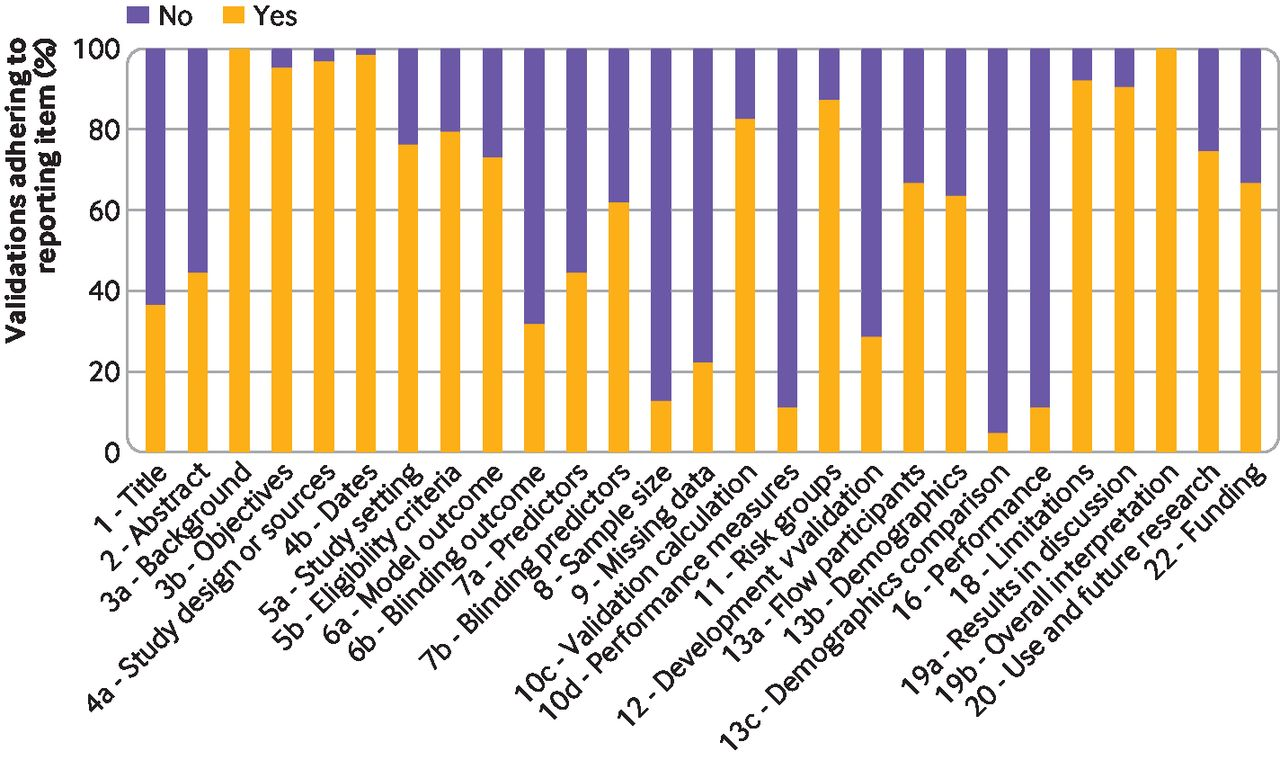
\includegraphics[width=0.8\textwidth]{figures/ADNEXSR/F2.large.jpg}
\caption[Adherence to TRIPOD]{Adherence to reporting the TRIPOD (Transparent Reporting of a multivariable prediction model for Individual Prognosis Or Diagnosis) items in 63 validations.}
\label{fig:1:2}
\end{figure}

\begin{figure}
\centering
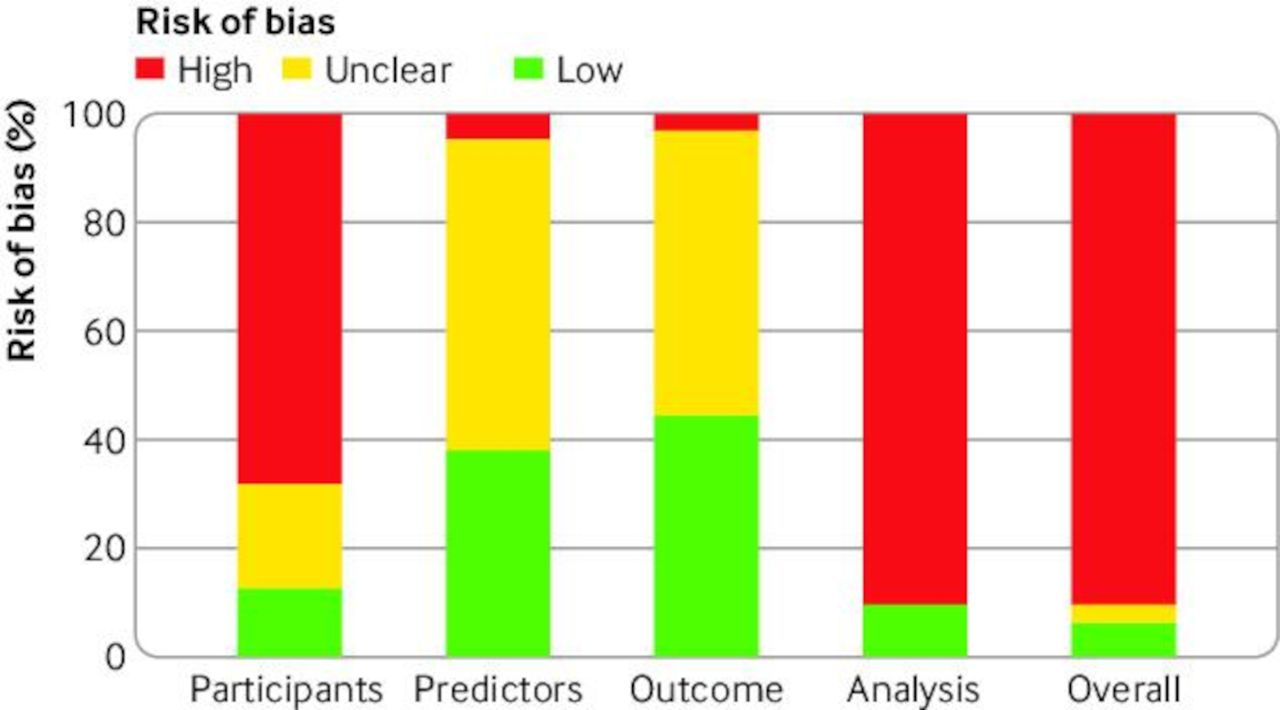
\includegraphics[width=0.8\textwidth]{figures/ADNEXSR/F3.large.jpg}
\caption[Risk of bias overall and by subdomain in 63 validations, assessed by PROBAST]{Risk of bias overall and by subdomain in 63 validations, assessed by PROBAST (Prediction model Risk Of Bias Assessment Tool).}
\label{fig:1:3}
\end{figure}
Fifty-seven (90\%) of 63 validations were rated at high risk of bias, two (3\%)
at uncertain risk of bias, and four (6\%) at low risk of bias (Figures \ref{fig:1:3}, S2-5,
\gls{OSF} Extraction sheet) \cite{barrenadaADNEXRiskModel2025}. 43 (68\%) validations
were at high risk of bias for the participant domain, mostly by having
incomplete data as an exclusion criterion. Fifty-seven (90\%) validations were
at high risk of bias for the analysis domain, mostly due to small sample size
(69\%; i.e. less than 100 tumours in the smallest group), not including all
participants in the analysis (85\%), inappropriate handling of missing data
(82\%), and incomplete evaluation of model performance - in most instances by
not reporting an assessment of calibration (89\%).

\gls{TRIPOD} adherence in 36 studies without focus on selected histologies or clinical
subgroups was on average 65\% (17.47 items out of 27). In these studies, two
where at low risk of bias, one at unclear risk of bias and 33 at high risk of
bias.

\subsection{Meta-analysis}
The meta-analysis included studies without post hoc selection based on histology
and without focus on a clinical subgroup only (n = 36) that reported the
meta-analysed metrics. Just two studies included in the meta-analysis used
tumour as unit of study
 \cite{behnamfarComparisonUltrasoundTumor2022,esquivelvillabonaTwoStepStrategyOptimizing2022}.

The \gls{AUC} for benign vs malignant tumours in operated patients was reported in 12
studies (6309 tumours, 31 centres, 13 countries) for \gls{ADNEX} without CA125 (Table
S4 and S6), and the summary \gls{AUC} was 0.93 (\gls{CI} 95\% 0.91-0.94, 95\% \gls{PI} 0.85-0.98)
(Table \ref{tab:2}, Figure \ref{fig:1:4})
 \cite{vancalsterValidationModelsDiagnose2020,chenComparisonORADSADNEX2022,
  diazOvarianTumorsRisk2017a,heEstimatingRiskMalignancy2021,
  hiettPerformanceIOTASimple2022,lamhuongOptimalCutOffPoint2022,
  pelayoComparisonUltrasoundScores2023,pengEvaluationDiagnosticValue2021,
  poonyakanokPreoperativeEvaluationADNEX2021,
  qianComparisonDiagnosticPerformances2021,
  sayasnehEvaluatingRiskOvarian2016,
  zhangExternalValidationAssessment2022}.
Twenty-one studies (9202 tumours, 43 centres, 18 countries) reported the \gls{AUC} for
benign vs malignant tumours in operated patients for \gls{ADNEX} with CA125,
 \cite{vancalsterValidationModelsDiagnose2020,araujoPerformanceIOTAADNEX2017,
  behnamfarComparisonUltrasoundTumor2022,chenPerformanceIOTAADNEX2019,
  diazOvarianTumorsRisk2017a,heEstimatingRiskMalignancy2021,
  joyeuxSurgeryPredictabilityMalignant2016,
  lamhuongOptimalCutOffPoint2022,meysEstimatingRiskMalignancy2017,
  namAssessmentDifferentNEoplasias2021,pengEvaluationDiagnosticValue2021,
  poonyakanokPreoperativeEvaluationADNEX2021,
  qianComparisonDiagnosticPerformances2021,
  sayasnehEvaluatingRiskOvarian2016,stukanDevelopmentValidationModel2019,
  szubertPerformanceSelectedModels2020,szubertExternalValidationIOTA2016,
  tugPreoperativeDiscriminatingPerformance2020,vioraADNEXModelTriage2020,
  yangPerformanceIOTAADNEX2022,zhangExternalValidationAssessment2022}
(Table S4 and S6) and the summary \gls{AUC} was 0.93 (\gls{CI} 95\% 0.92-0.94, 95\% \gls{PI}
0.85-0.98) (Table \ref{tab:2}, Figure \ref{fig:1:5}).

\begin{figure}
\flushleft
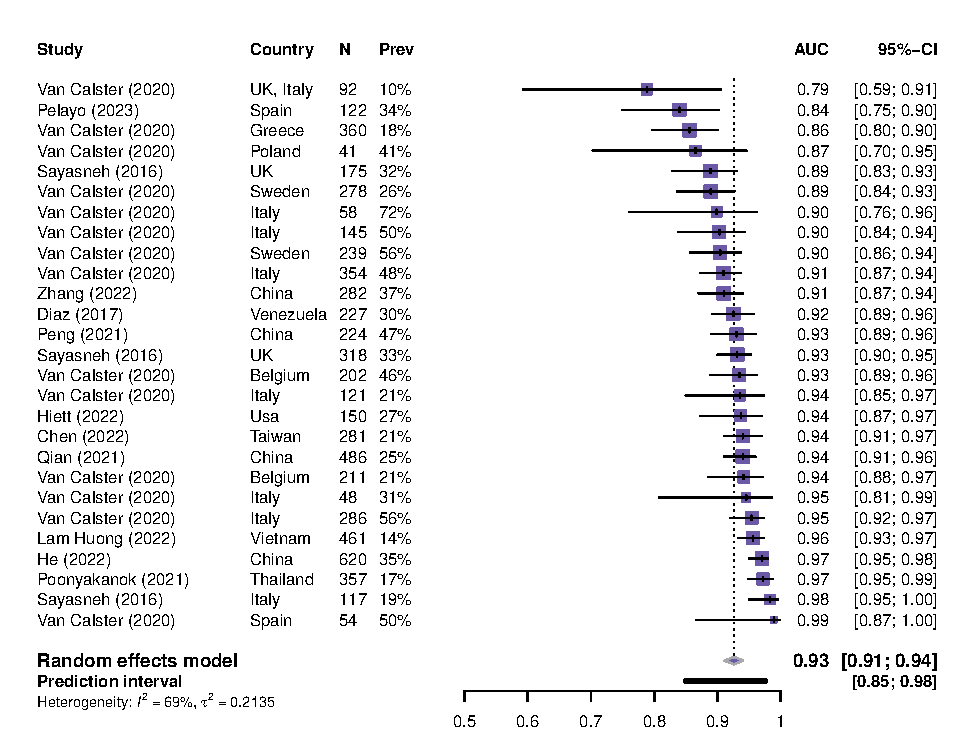
\includegraphics[width=1\textwidth]{figures/ADNEXSR/Figure4.pdf}
\caption[Forest plot AUC ADNEX without CA125]{Forest plot of area under the receiver operating curve in studies where the ADNEX (Assessment of Different Neoplasias in the adnexa) model was used without CA125 (cancer antigen 125). Results in the forest plot are centre specific results, so studies with more than one centre can appear multiple times. CI=confidence interval}
\label{fig:1:4}
\end{figure}

\begin{figure}
\flushleft
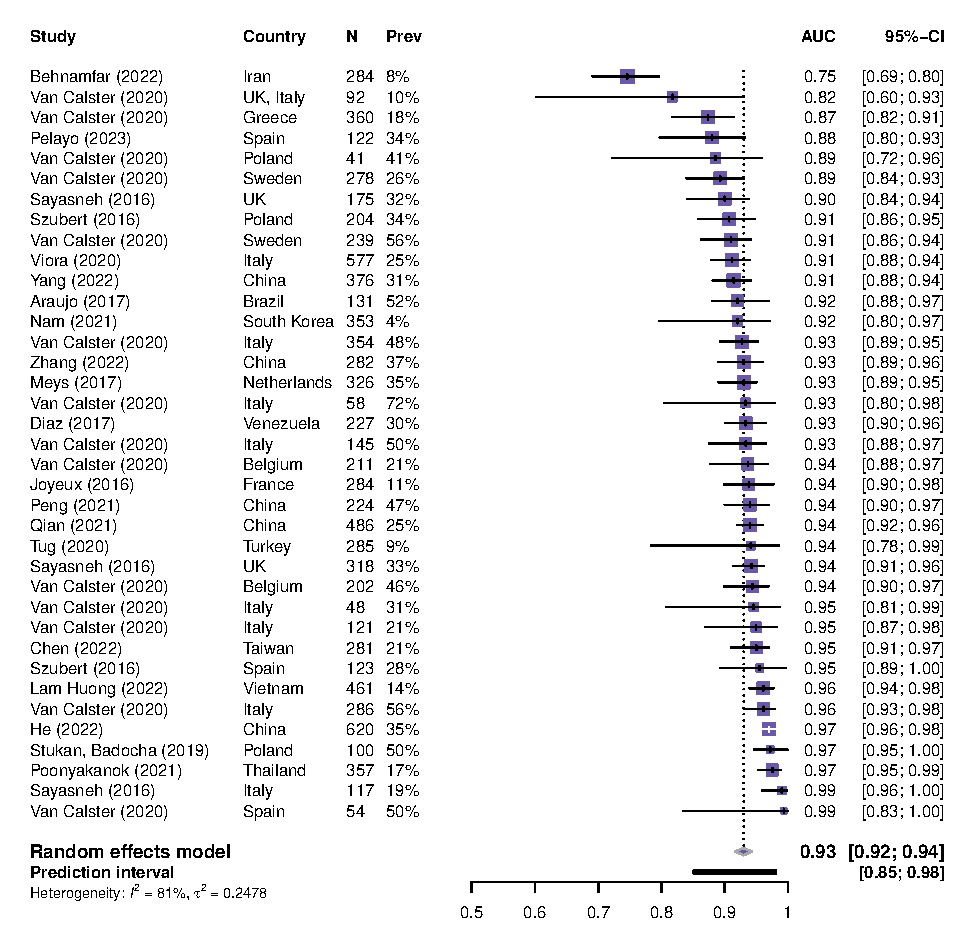
\includegraphics[width=1\textwidth]{figures/ADNEXSR/Figure5.pdf}
\caption[Forest plot AUC ADNEX with CA125]{Forest plot of area under the receiver operating characteristic curve in studies where the ADNEX (Assessment of Different Neoplasias in the adnexa) model was used with CA125 (cancer antigen 125). Results in the forest plot are centre specific results, so studies with more than one centre can appear multiple times. CI=confidence interval}
\label{fig:1:5}
\end{figure}




Sensitivity and specificity at the 10\% risk of malignancy threshold in operated
patients were reported in ten studies for \gls{ADNEX} without CA125 (Tables S4 and S7)
 \cite{vancalsterValidationModelsDiagnose2020,chenComparisonORADSADNEX2022,
  diazOvarianTumorsRisk2017a,hiettPerformanceIOTASimple2022,
  lamhuongOptimalCutOffPoint2022,pelayoComparisonUltrasoundScores2023,
  poonyakanokPreoperativeEvaluationADNEX2021,
  qianComparisonDiagnosticPerformances2021,
  sayasnehEvaluatingRiskOvarian2016,
  zhangExternalValidationAssessment2022}.
The summary sensitivity and specificity were 0.93 (95\% \gls{CI} 0.90-0.95, 95\% \gls{PI}
0.73-0.99) and 0.75 (95\% \gls{CI} 0.70-0.79, 95\% \gls{PI} 0.46-0.91), respectively (Table
S8, Figure \ref{fig:1:6}). For \gls{ADNEX} with CA125, sensitivity and specificity at the 10\%
risk of malignancy threshold in operated patients were reported in 24 studies
(Tables S4 and S7)
 \cite{vancalsterValidationModelsDiagnose2020,
  jeongValidationIOTAADNEXModel2020,araujoPerformanceIOTAADNEX2017,
  chenComparisonORADSADNEX2022,diazOvarianTumorsRisk2017a,
  heEstimatingRiskMalignancy2021,
  joyeuxSurgeryPredictabilityMalignant2016,laiComparisonORADSGIRADS2022,
  lamhuongOptimalCutOffPoint2022,meysEstimatingRiskMalignancy2017,
  namAssessmentDifferentNEoplasias2021,
  pelayoComparisonUltrasoundScores2023,pengEvaluationDiagnosticValue2021,
  poonyakanokPreoperativeEvaluationADNEX2021,
  qianComparisonDiagnosticPerformances2021,
  sandalComparisionRiskMalignancy2018a,sayasnehEvaluatingRiskOvarian2016,
  stukanDevelopmentValidationModel2019,szubertExternalValidationIOTA2016,
  tugPreoperativeDiscriminatingPerformance2020,vioraADNEXModelTriage2020,
  wangEvaluatingRiskMalignancy2023,yangPerformanceIOTAADNEX2022,
  zhangExternalValidationAssessment2022}.
The summary sensitivity and specificity were 0.94 (\gls{CI} 95\% 0.92-0.95; 95\% \gls{PI}
0.80-0.98) and 0.77 (\gls{CI} 95\% 0.73-0.81; 95\% \gls{PI} 0.47-0.93, respectively (Table
S8, Figure \ref{fig:1:7}).

\gls{NB} and \gls{RU} were calculated using studies that presented sensitivity and
specificity at the 10\% risk of malignancy threshold in operated patients (Table
S7). For \gls{ADNEX} without CA125, the summary \gls{NB} was 0.28 (95\% \gls{CrI} 0.22-0.35, 95\%
\gls{PI} 0.05-0.67) and the summary \gls{RU} 0.50 (95\% \gls{CrI} 0.36-0.62, 95\% \gls{PI} -0.41-0.81).
The probability that the model is clinically useful in a random new centre was
estimated to be 91\% (Table S9, Figures S6-7). For \gls{ADNEX} with CA125, the summary
\gls{NB} was 0.27 (95\% \gls{CrI} 0.23-0.33, 95\% \gls{PI} 0.06-0.64) and the summary \gls{RU} 0.54
(95\% \gls{CrI} 0.45-0.61, 95\% \gls{PI} -0.12-0.78). The probability that the model is
clinically useful in a random new centre was estimated to be 95\% (Table S9,
Figures S8-9).

Pairwise \glspl{AUC} in operated patients were reported in 4 studies for \gls{ADNEX} without
CA125 and in 5 studies for \gls{ADNEX} with CA125 (Table S10)
 \cite{vancalsterValidationModelsDiagnose2020,
  poonyakanokPreoperativeEvaluationADNEX2021,
  sayasnehEvaluatingRiskOvarian2016,vioraADNEXModelTriage2020,
  zhangExternalValidationAssessment2022}.
The summary pairwise \glspl{AUC} for \gls{ADNEX} without CA125 ranged from 0.66 (stage II-IV
primary invasive vs metastatic) to 0.97 (benign vs stage II-IV primary invasive)
(Table S11). For \gls{ADNEX} with CA125, the summary pairwise \glspl{AUC} ranged from 0.72
(borderline vs stage I primary invasive) to 0.98 (benign vs stage II-IV primary
invasive).

\begin{figure}
\flushleft
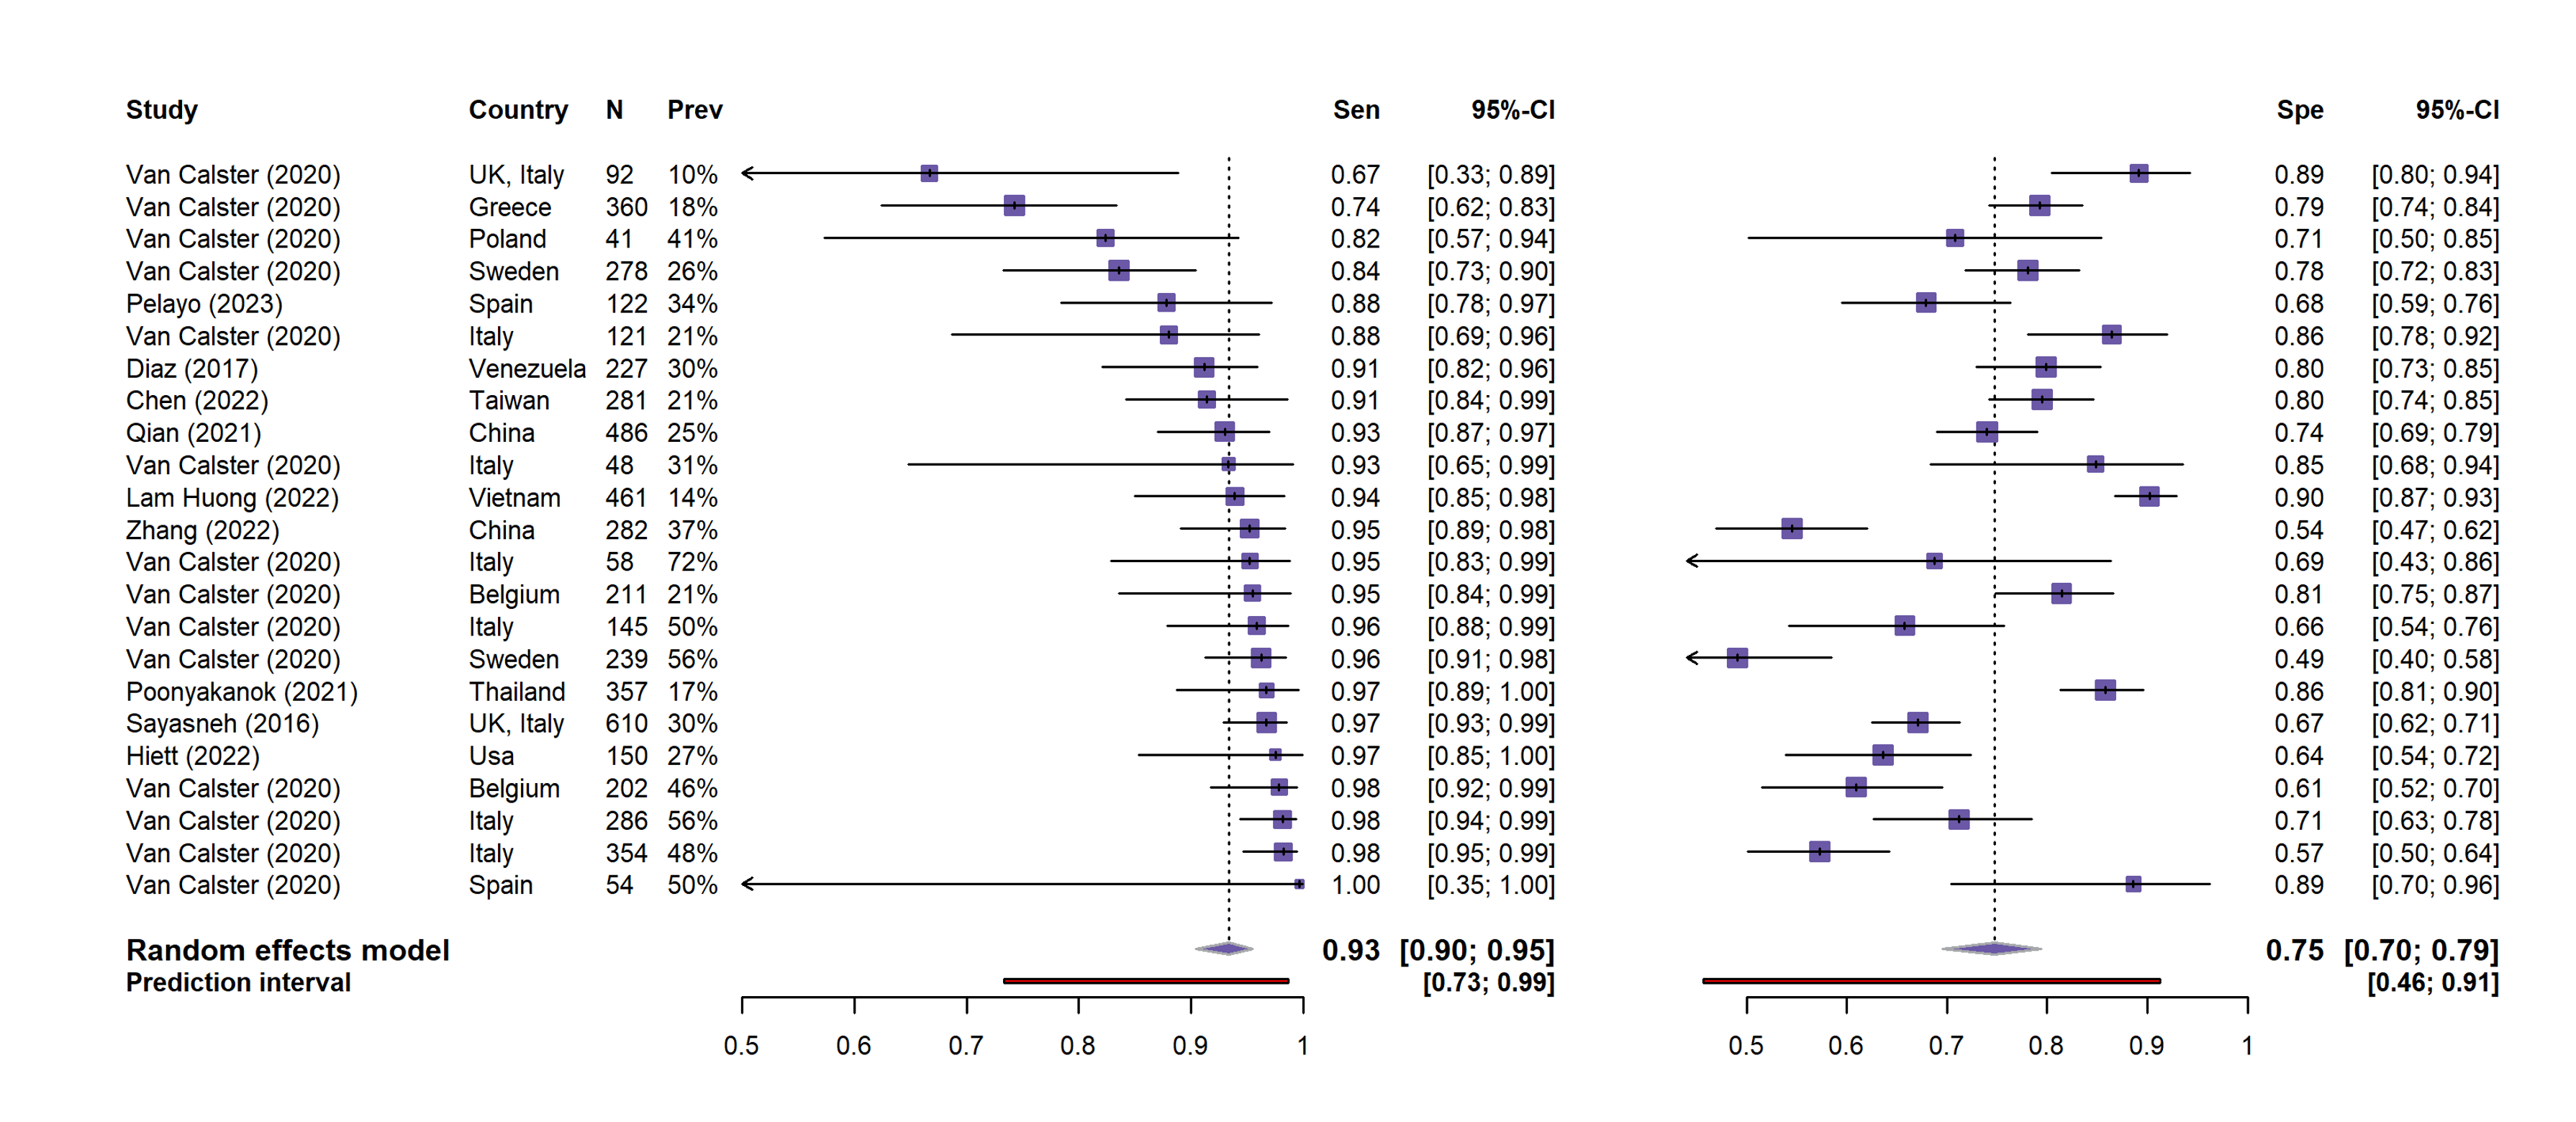
\includegraphics[width=1\textwidth]{figures/ADNEXSR/Figure6.png}
\caption[Forest plot sensitivity and specificity ADNEX without CA125 at 10\% risk of malignancy]{Forest plot of sensitivity and specificity at the 10\% risk of malignancy threshold in studies where the ADNEX (Assessment of Different Neoplasias in the adnexa) model was used without CA125 (cancer antigen 125). Results in the forest plot are centre specific results, so studies with more than one centre can appear multiple times. CI=confidence interval}
\label{fig:1:6}
\end{figure}

The \gls{AUC} for benign vs malignant tumours in operated and non-surgically managed
patients combined was reported in 2 studies (5167 tumours, 18 centres, 8
countries) with a summary estimate of 0.94 (95\% \gls{CI} 0.93-0.96, 95\% \gls{PI}
0.88-0.99) for \gls{ADNEX} with CA125 (Table \ref{tab:2})
 \cite{vancalsterValidationModelsDiagnose2020,hackExternalValidationORADS2022}.
\gls{ADNEX} without CA125 was assessed in only 1 study (4905 tumours, 17 centres, 7
countries) \cite{vancalsterValidationModelsDiagnose2020}. This study reported
summary \gls{AUC} 0.94 (95\% \gls{CI} 0.91-0.95, 95\% \gls{PI} 0.82-0.98).

Sensitivity and subgroup results for \gls{AUC}, specificity, sensitivity, \gls{NB} and \gls{RU}
are shown in Tables 2 and S6-9. These results showed that findings were robust
(\glspl{AUC} ranged from 0.90 to 0.95 across all analyses) and clinical utility was
suggested in all subgroups. When limiting the analyses to low RoB studies,
summary \glspl{AUC} were 0.93 (with CA125) and 0.91 (without CA125). Sensitivity was
higher and specificity lower in oncology versus non-oncology centres and in
postmenopausal versus premenopausal patients. In line with this, meta-regression
suggested that prevalence of malignancy was not related to \gls{AUC} but positively to
sensitivity and negatively to specificity (Figures S10-12).

\begin{figure}
\flushleft
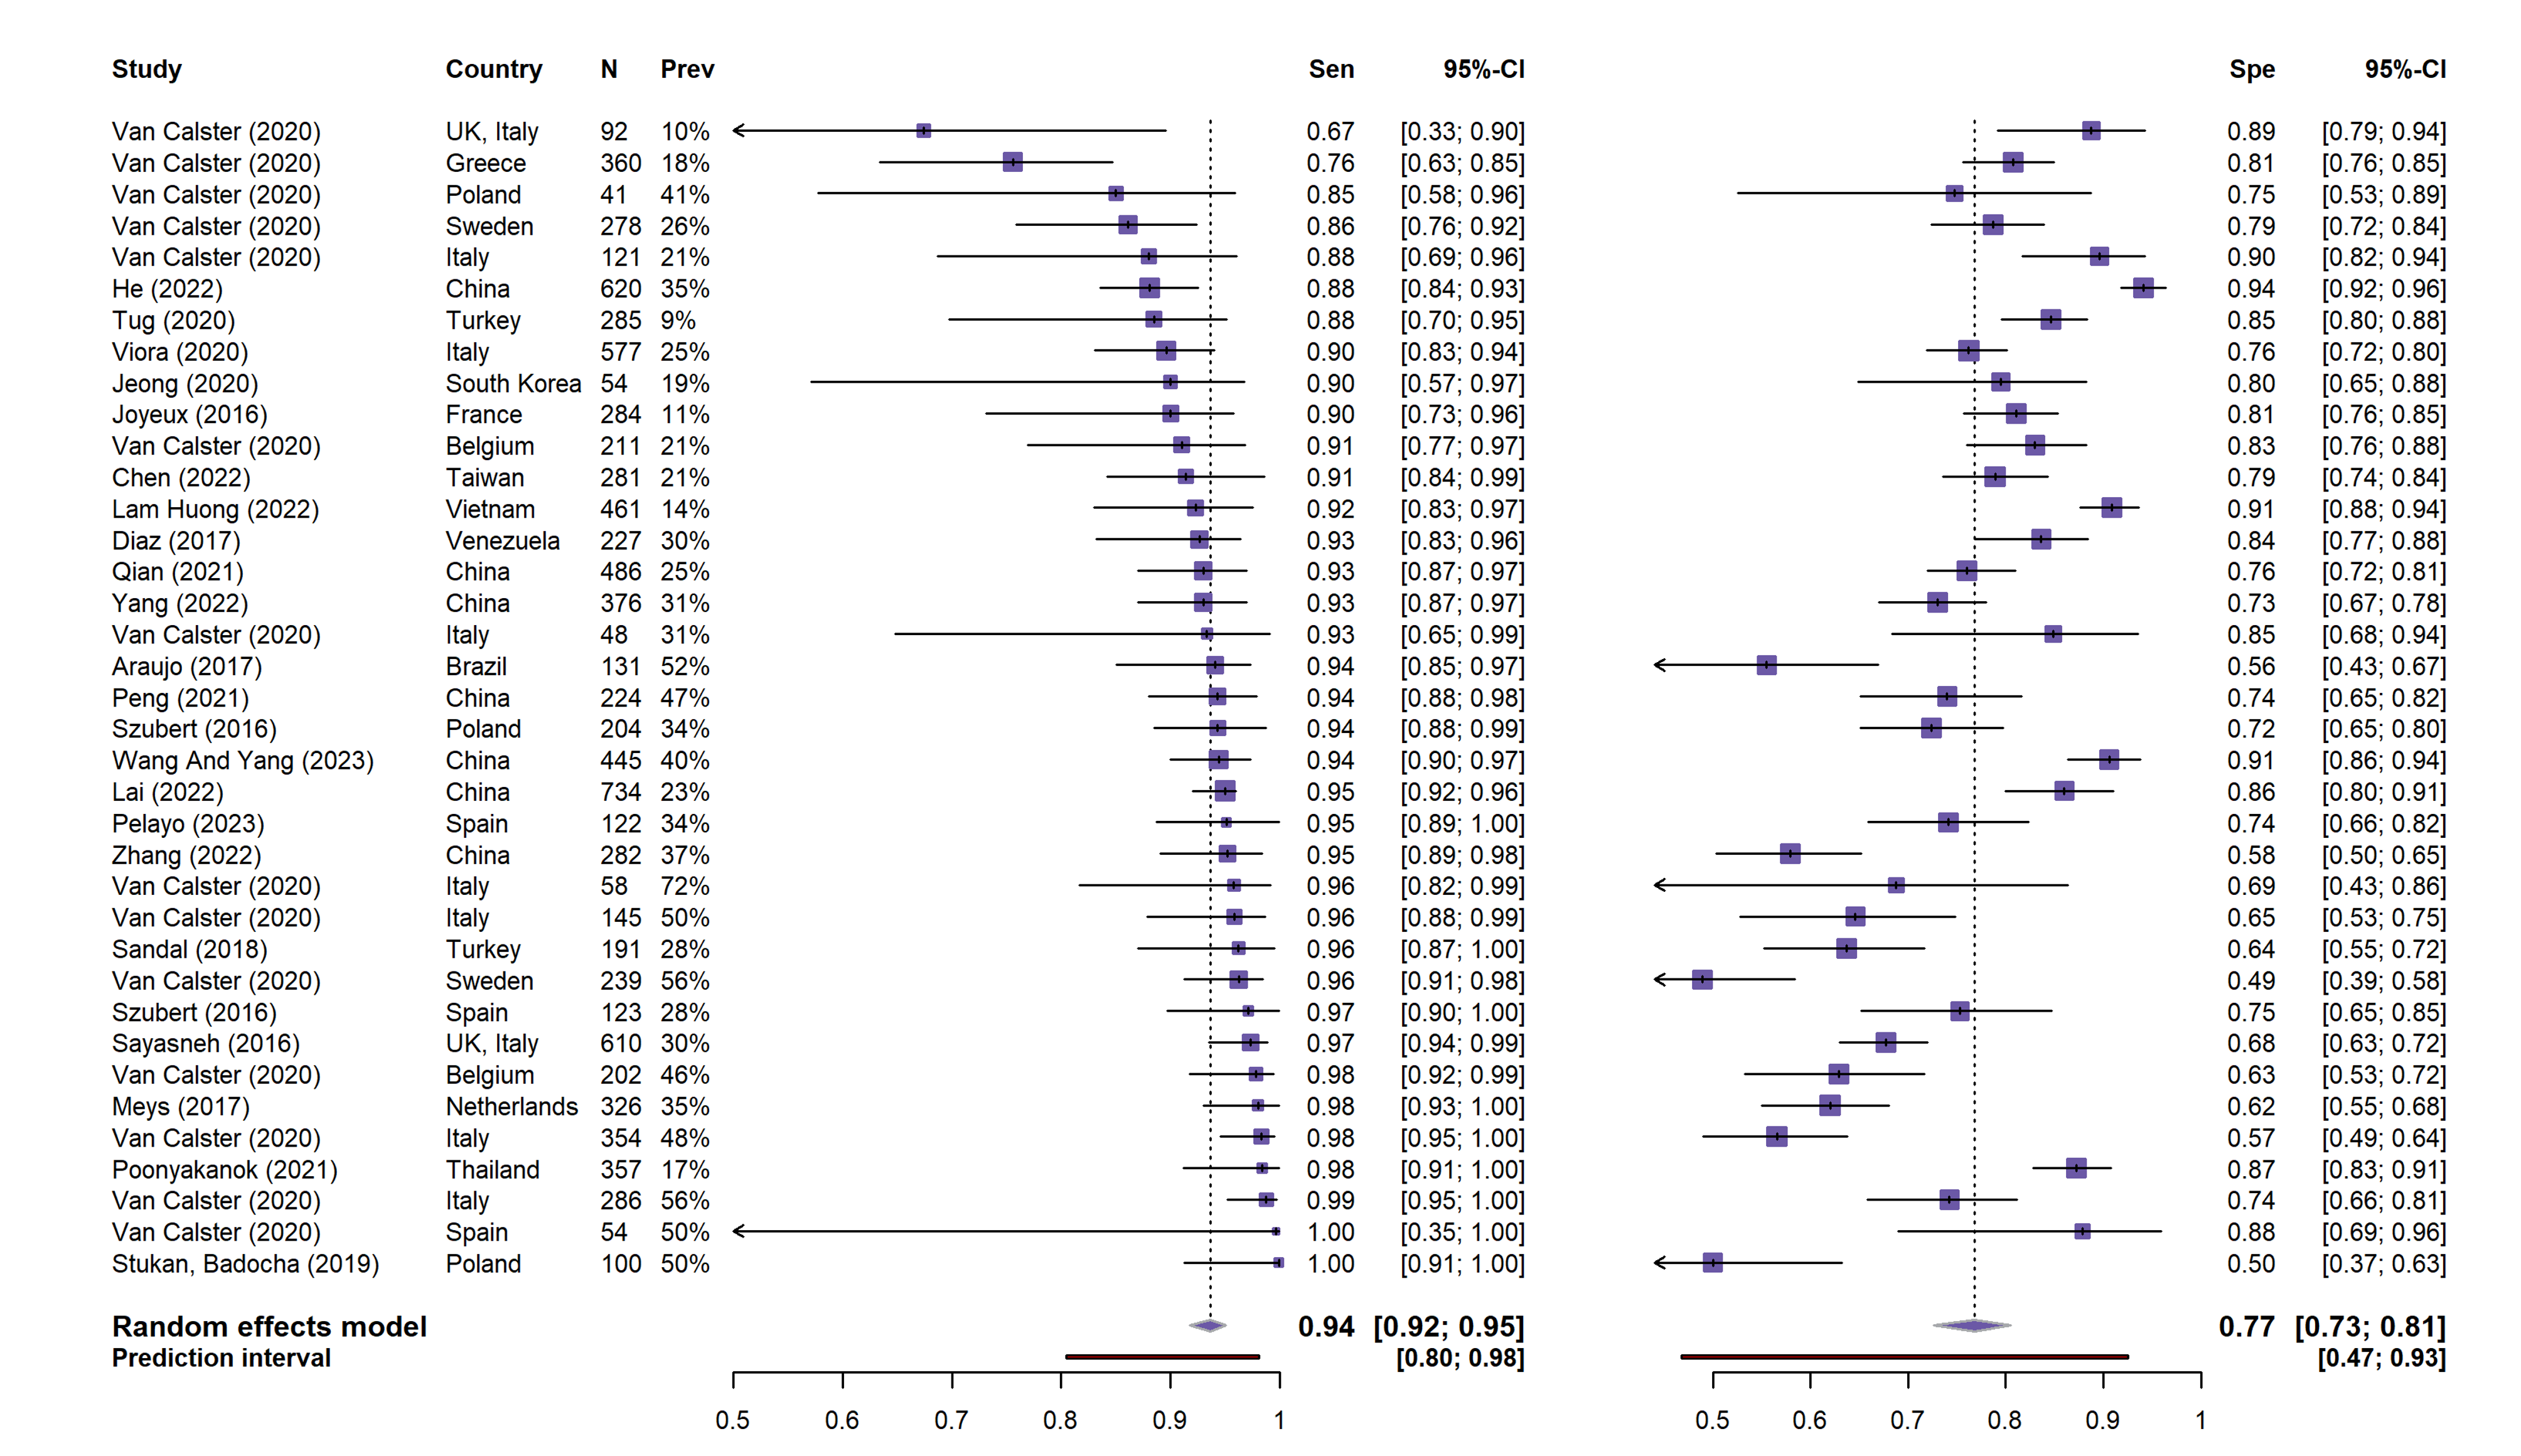
\includegraphics[width=1\textwidth]{figures/ADNEXSR/Figure7.png}
\caption[Forest plot sensitivity and specificity ADNEX with CA125 at 10\% risk of malignancy]{Forest plot of sensitivity and specificity at the 10\% risk of malignancy threshold in studies where the ADNEX (Assessment of Different Neoplasias in the adnexa) model was used with CA125 (cancer antigen 125). Results in the forest plot are centre specific results, so studies with more than one centre can appear multiple times. CI=confidence interval}
\label{fig:1:7}
\end{figure}



Meta-analysis of calibration in only operated patients was not feasible as only
one study reported calibration slope and intercept
 \cite{vancalsterValidationModelsDiagnose2020}. Four studies presented a
calibration plot: in three studies
 \cite{sayasnehEvaluatingRiskOvarian2016,vioraADNEXModelTriage2020,zhangExternalValidationAssessment2022}
the estimated risks were close to the observed ones, in one study
 \cite{vancalsterValidationModelsDiagnose2020} the risk of malignancy was
slightly underestimated (Supplementary material S8).

Based on the subdomains of \gls{GRADE} assessment, we have identified the risk of bias
in the studies included in this meta-analysis as a significant limitation
affecting the certainty of our meta-analysis results. Two studies (representing
5511 tumours or 32\% of total tumours included in this review) did not fall
under the classification of high risk of bias
 \cite{vancalsterValidationModelsDiagnose2020,sayasnehEvaluatingRiskOvarian2016}.
However, the sensitivity analysis according to risk of bias showed consistent
findings (Table \ref{tab:2}, Table S8 and S9). Funnel plots for the \gls{AUC} did not suggest
publication bias (Figure S13).

\section{Discussion}

The \gls{ADNEX} model exhibited robust discrimination and classification performance
between benign and malignant tumours across various settings and populations. In
addition, the results indicate that \gls{ADNEX} has clinical utility at the 10\% risk
of malignancy threshold, for example to help decide whether a patient should be
referred for assessment in a gynaecological oncology centre.

We found deficiencies in study reporting, and most studies were judged to be at
high risk of bias. However, our sensitivity analyses indicated that performance
was almost identical in low risk and high risk of bias studies. For \gls{ADNEX} with
CA125, the \gls{AUC} was 0.93 based on all studies vs 0.93 when based on only low risk
of bias studies. For \gls{ADNEX} without CA125, the \glspl{AUC} were 0.93 (all studies) and
0.91 (low risk of bias only). High risk of bias was mainly caused by low sample
size, absence of calibration performance, and unjustified use of complete case
analysis. Low sample size makes the estimated \gls{AUC} less precise but does not
systematically affect the \gls{AUC}, unless there is publication bias. The funnel
plots do not suggest publication bias. Absence of calibration does not affect
the \gls{AUC}. Using complete cases regarding CA125 or other predictors may lead to
underestimation of the \gls{AUC}, because missing values tend to be associated with
the examiner’s subjective impression that the tumour is benign
 \cite{landolfoBenignDescriptorsADNEX2023}. Complete case analysis would then
tend to exclude clearly benign tumours, which would make the sample more
homogeneous and reduce the \gls{AUC}. However, our results suggest that the impact of
complete case analysis on performance may have been minimal. The impact on
calibration could not be assessed. Taken together, the results presented in our
meta-analysis are reliable.

Strengths of our systematic review include the meta-analysis of \gls{ADNEX} both as a
risk model and as a diagnostic test, and the thorough critical appraisal
regarding risk of bias and reporting quality using recommended checklists
 \cite{wolffPROBASTToolAssess2019,collinsTransparentReportingMultivariable2015}.
Our study also has limitations. First, some study authors have a conflict of
interest because they were involved in developing \gls{ADNEX} or in some of the
included external validation studies. To address this, independent researchers
with expertise in study methodology and prediction modelling evaluated the
\gls{IOTA}-related studies. A limitation of our findings (but not of our study) is
that calibration performance was reported in only four studies so that
meta-analysis of calibration was not possible.

Previous systematic reviews have conducted meta-analyses of the diagnostic
performance of \gls{ADNEX} with CA125
 \cite{cuiDiagnosticAccuraciesUltrasound2022,
  davenportMenopausalStatusUltrasound2022,
  huangDiagnosticAccuracyADNEX2021,westwoodRiskScoresGuide2018,
  yueValueAssessmentDifferent2022}.
They used the \gls{QUADAS}-2 tool \cite{whitingQUADAS2RevisedTool2011} to assess risk
of bias, and found between 0 and 64\% of studies to be at high risk of bias in
at least one domain. We identified 45/47 studies as high risk of bias using the
\gls{PROBAST} tool designed for the appraisal of risk prediction models. None of the
previous meta-analyses of \gls{ADNEX} included clinical utility, calibration or \gls{AUC}.
Our results align with those of other systematic reviews of risk prediction
modelling studies in various domains. These consistently indicate that reporting
in the original studies was poor and that many studies were at high risk of bias
 \cite{collinsExternalValidationMultivariable2014,
  wynantsPredictionModelsDiagnosis2020,
  helmrichDoesPoorMethodological2022,
  dhimanReportingPrognosticClinical2021,andaurnavarroRiskBiasStudies2021,
  alloteyExternalValidationPrognostic2022,
  bouwmeesterReportingMethodsClinical2012}.
Still, the results in terms of sensitivity and specificity of \gls{ADNEX} in our
meta-analysis were similar to those in the other meta-analyses of \gls{ADNEX}
performance.

\gls{ADNEX} is intended for use by gynaecologists to help them decide on the most
appropriate management of an adnexal mass detected on ultrasound. Our findings
support the use of \gls{ADNEX} (1) to choose between surgery and conservative
follow-up, the latter in case of very low risk of malignancy, e.g. < 1\%
(meta-analysis in operated and non-surgically managed patients) (2) to decide on
the most appropriate management if conservative management is not suitable, e.g.
surgery at a local hospital if the risk of malignancy is less than 10\% or
referral to an oncology centre if the risk is >10\% (meta-analysis in operated
patients) \cite{timmermanESGOISUOGIOTA2021}. \gls{ADNEX} can also be helpful when
deciding on management of a suspected malignancy, i.e. investigations to find
the primary tumour if a metastasis in the ovary is likely, or fertility sparing
surgery if a borderline tumour is likely (meta-analysis in operated patients).
Because the \gls{AUC} of \gls{ADNEX} with and without CA125 are similar, and because adding
CA125 mainly helps to distinguish between different types of malignant tumours,
we argue that the main use of \gls{ADNEX} without CA125 is to help decide whether
conservative follow-up, surgery in a local centre or referral to an oncology
centre is appropriate. The main use of \gls{ADNEX} with CA125 is to help decide on
optimal management of a tumour suspected to be malignant, because it
differentiates better between malignant subtypes than \gls{ADNEX} without CA125.

While our findings suggest that \gls{ADNEX} has clinically utility, well conducted
validations of any model are always of value to monitor its performance in
diverse regions and clinical settings, and over time
 \cite{vancalsterThereNoSuch2023}. In line with this, to improve \gls{ADNEX}
performance even further, efforts to update the \gls{ADNEX} formula are of interest
 \cite{vancalsterThereNoSuch2023,
  onbehalfoftopicgroupevaluatingdiagnostictestsandpredictionmodelsofthestratosinitiativeCalibrationAchillesHeel2019}.
If further validation studies are conducted, we recommend to include a
validation of \gls{ADNEX} without CA125, to use a sufficiently large sample that
allows to assess calibration and multinomial discrimination, and to include
patients irrespective of whether they are managed surgically or non-surgically
(despite the challenges regarding reference standard for non-surgically managed
patients)
 \cite{vancalsterAssessingDiscriminativeAbility2012,vanhoordeAssessingCalibrationMultinomial2014}.
Methodological recommendations for validation studies include using available
tools to guarantee adequate sample size, describe missing data in detail and use
methods such as imputation when needed, and assess calibration performance
 \cite{steyerbergClinicalPredictionModels2009,
  onbehalfoftopicgroupevaluatingdiagnostictestsandpredictionmodelsofthestratosinitiativeCalibrationAchillesHeel2019,
  pateMinimumSampleSize2023,rileyMinimumSampleSize2021,
  siskImputationMissingIndicators2023}.
Finally, adherence to the \gls{TRIPOD} reporting checklists is important to maximise
the value of the validation study (www.tripod-statement.org).

\section{Conclusion}
\gls{ADNEX} has been widely validated with \gls{AUC} values >0.90 to discriminate between
benign and malignant tumours across various settings, and with strong results
regarding clinical utility at the 10\% risk of malignancy threshold. Due to lack
of calibration assessment in most studies, it was not possible to substantially
evaluate the accuracy of the estimated risks.

\section*{Acknowledgment}
The authors wish to thank Thomas Vandendriessche, Chayenne Van Meel and Krizia
Tuand, the biomedical reference librarians of the KU Leuven Libraries – 2Bergen
– learning Centre Désiré Collen (Leuven, Belgium), for their help in conducting
the systematic literature search. We gratefully acknowledge the authors of the
external validation of \gls{ADNEX} for providing their valuable data. This research
will be presented at \gls{ISUOG} World Congress 2023 in Seoul (October 2023).

\section*{Other information}
\subsection*{Funding}
This research was supported by the Research Foundation – Flanders (FWO) under
grant G097322N with BVC and DT as supervisors. LW and BVC were supported by
Internal Funds KU Leuven (grant C24M/20/064). JYV was supported by the National
Institute for Health and Care Research (NIHR) Community Healthcare MedTech and
In Vitro Diagnostics Co-operative at Oxford Health NHS Foundation Trust (N/A).
The views expressed are those of the author(s) and not necessarily those of the
NHS, the NIHR or the Department of Health and Social Care. GSC is supported by
Cancer Research UK (programme grant: C49297/A27294). PD is supported by CRUK
(project grant: PRCPJT-Nov21\textbackslash100021).

\subsection*{Conflicts of interest}
All authors have completed the ICMJE uniform disclosure form at
www.icmje.org/coi\_disclosure.pdf and declare: BVC, LV and DT are members of the
steering committee of the International Ovarian Tumour Analysis (\gls{IOTA})
consortium and were involved in the development of the \gls{ADNEX} model. BVC and DT
report consultancy work done by KU Leuven to help implementing and testing the
\gls{ADNEX} model in ultrasound machines by Samsung Medison, GE Healthcare, Canon
Medical Systems Europe, and Shenzhen Mindray Bio-medical Electronics, outside
the submitted work. GSC is a statistics editor for the BMJ. AL, LB, PD, LW and
JYV have nothing to declare.

\subsection*{Transparency declaration}
The lead authors affirm that this manuscript is an honest, accurate, and
transparent account of the study being reported; that no important aspects of
the study have been omitted; and that any discrepancies from the study as
planned (and, if relevant, registered) have been explained.

\subsection*{Availability of data and code}
Supplementary material is available online \cite{barrenadaADNEXRiskPrediction2024}.
The data and code used for the analysis and the generation of the figures is
publicly available in Open Science Framework (\url{https://osf.io/jtsvd/})
 \cite{barrenadaADNEXRiskModel2025}. This includes the extraction sheet, one
script for running the meta-analysis and one script for generating all the
figures included in the paper (except \gls{PRISMA} Flowchart). Note that for some rows
in the extraction sheet we deleted the performance measures for the menopausal
subgroups because this information was provided by authors upon request
therefore it is not publicly available.

\subsection*{Contributors}
Contributions were based on the CRediT taxonomy. Conceptualization: LB, BVC.
Funding acquisition: BVC, DT. Project administration: LB. Supervision: BVC.
Methodology: LB, GSC, LW, JYV, BVC. Resources: LB, AL. Investigation: LB, AL,
LV, BVC. Validation: LB, AL, PD, GSC, BVC. Data curation: LB, AL, JYV, LV, BVC.
Software: LB, LW, BVC. Formal analysis: LB, LW, BVC. Visualization: LB. Writing
– original draft: LB, BVC. Writing – review \& editing: all authors. All authors
have read, share final responsibility for the decision to submit for
publication, and agree to be accountable for all aspects of the work.

\subsection*{Ethics approval}
Not required because only secondary data from published studies were used.
